\PassOptionsToPackage{unicode=true}{hyperref} % options for packages loaded elsewhere
\PassOptionsToPackage{hyphens}{url}
%
\documentclass[english,man,floatsintext]{apa6}
\usepackage{lmodern}
\usepackage{amssymb,amsmath}
\usepackage{ifxetex,ifluatex}
\usepackage{fixltx2e} % provides \textsubscript
\ifnum 0\ifxetex 1\fi\ifluatex 1\fi=0 % if pdftex
  \usepackage[T1]{fontenc}
  \usepackage[utf8]{inputenc}
  \usepackage{textcomp} % provides euro and other symbols
\else % if luatex or xelatex
  \usepackage{unicode-math}
  \defaultfontfeatures{Ligatures=TeX,Scale=MatchLowercase}
\fi
% use upquote if available, for straight quotes in verbatim environments
\IfFileExists{upquote.sty}{\usepackage{upquote}}{}
% use microtype if available
\IfFileExists{microtype.sty}{%
\usepackage[]{microtype}
\UseMicrotypeSet[protrusion]{basicmath} % disable protrusion for tt fonts
}{}
\IfFileExists{parskip.sty}{%
\usepackage{parskip}
}{% else
\setlength{\parindent}{0pt}
\setlength{\parskip}{6pt plus 2pt minus 1pt}
}
\usepackage{hyperref}
\hypersetup{
            pdftitle={Extended Wireless pH monitoring significantly increases GORD diagnoses in patients with a negative pH impedance study but can be difficult to predict.},
            pdfkeywords={Gastro-oesophageal reflux disease, pH studies, wireless pH monitoring},
            pdfborder={0 0 0},
            breaklinks=true}
\urlstyle{same}  % don't use monospace font for urls
\usepackage{graphicx,grffile}
\makeatletter
\def\maxwidth{\ifdim\Gin@nat@width>\linewidth\linewidth\else\Gin@nat@width\fi}
\def\maxheight{\ifdim\Gin@nat@height>\textheight\textheight\else\Gin@nat@height\fi}
\makeatother
% Scale images if necessary, so that they will not overflow the page
% margins by default, and it is still possible to overwrite the defaults
% using explicit options in \includegraphics[width, height, ...]{}
\setkeys{Gin}{width=\maxwidth,height=\maxheight,keepaspectratio}
\setlength{\emergencystretch}{3em}  % prevent overfull lines
\providecommand{\tightlist}{%
  \setlength{\itemsep}{0pt}\setlength{\parskip}{0pt}}
\setcounter{secnumdepth}{0}

% set default figure placement to htbp
\makeatletter
\def\fps@figure{htbp}
\makeatother

% Manuscript styling
\usepackage{upgreek}
\captionsetup{font=singlespacing,justification=justified}

% Table formatting
\usepackage{longtable}
\usepackage{lscape}
% \usepackage[counterclockwise]{rotating}   % Landscape page setup for large tables
\usepackage{multirow}		% Table styling
\usepackage{tabularx}		% Control Column width
\usepackage[flushleft]{threeparttable}	% Allows for three part tables with a specified notes section
\usepackage{threeparttablex}            % Lets threeparttable work with longtable

% Create new environments so endfloat can handle them
% \newenvironment{ltable}
%   {\begin{landscape}\begin{center}\begin{threeparttable}}
%   {\end{threeparttable}\end{center}\end{landscape}}
\newenvironment{lltable}{\begin{landscape}\begin{center}\begin{ThreePartTable}}{\end{ThreePartTable}\end{center}\end{landscape}}

% Enables adjusting longtable caption width to table width
% Solution found at http://golatex.de/longtable-mit-caption-so-breit-wie-die-tabelle-t15767.html
\makeatletter
\newcommand\LastLTentrywidth{1em}
\newlength\longtablewidth
\setlength{\longtablewidth}{1in}
\newcommand{\getlongtablewidth}{\begingroup \ifcsname LT@\roman{LT@tables}\endcsname \global\longtablewidth=0pt \renewcommand{\LT@entry}[2]{\global\advance\longtablewidth by ##2\relax\gdef\LastLTentrywidth{##2}}\@nameuse{LT@\roman{LT@tables}} \fi \endgroup}

% \setlength{\parindent}{0.5in}
% \setlength{\parskip}{0pt plus 0pt minus 0pt}

% \usepackage{etoolbox}
\makeatletter
\patchcmd{\HyOrg@maketitle}
  {\section{\normalfont\normalsize\abstractname}}
  {\section*{\normalfont\normalsize\abstractname}}
  {}{\typeout{Failed to patch abstract.}}
\makeatother
\shorttitle{Extended Wireless pH monitoring significantly increases GORD diagnoses in patients with a negative pH impedancestudy but can be difficult to predict.}
\author{Sebastian S Zeki\textsuperscript{1,3}, Ismail Miah\textsuperscript{1}, Anna Wolak\textsuperscript{1}, Minerva daSilva\textsuperscript{1}, Jason Dunn\textsuperscript{1,2}, Andrew Davies\textsuperscript{1,2}, James Gossage\textsuperscript{1,2}, Abrie Botha\textsuperscript{1,2}, Guiping Sui\textsuperscript{1}, Jafar Jafari\textsuperscript{1}, \& Terry Wong\textsuperscript{1,2}}
\affiliation{
\vspace{0.5cm}
\textsuperscript{1} Centre for Oeosphageal Diseases, Guy's and St. Thomas Hospital, Westminster Bridge Road, London\\\textsuperscript{2} Karolinska Instituet, Karolinska,Sweden\\\textsuperscript{3} Bart's Cancer Institute,Charterhouse Square, London}
\authornote{

Correspondence concerning this article should be addressed to Sebastian S Zeki, Gastroenterology Department,Westminster Bridge Road, London SE1 7EH. E-mail: sebastiz@hotmail.com}
\keywords{Gastro-oesophageal reflux disease, pH studies, wireless pH monitoring\newline\indent Word count: This document contains 2301 words}
\usepackage{lineno}

\linenumbers
\usepackage{csquotes}
\usepackage{setspace}\doublespacing
\AtBeginEnvironment{tabular}{\singlespacing}
\AtBeginEnvironment{lltable}{\singlespacing}
\AtBeginEnvironment{tablenotes}{\doublespacing}
\captionsetup[table]{font={stretch=1.5}}
\captionsetup[figure]{font={stretch=1.5}}
\ifnum 0\ifxetex 1\fi\ifluatex 1\fi=0 % if pdftex
  \usepackage[shorthands=off,main=english]{babel}
\else
  % load polyglossia as late as possible as it *could* call bidi if RTL lang (e.g. Hebrew or Arabic)
  \usepackage{polyglossia}
  \setmainlanguage[]{english}
\fi

\title{Extended Wireless pH monitoring significantly increases GORD diagnoses in patients with a negative pH impedance study but can be difficult to predict.}

\date{}

\abstract{
Introduction: Patients often undergo assessment for the presence of gastro-oesophageal reflux as a cause of their symptoms. This is most often done by catheter based methods such as pH impedance and manometry if endoscopic evaluation is not diagnostic. In some patients a false negative catheter test may be suspected. Further testing can be done using a prolonged acid monitoring test such as the wireless pH monitoring (WPM) device which can assess acidic reflux for 96 hours. The increased yield of GORD-positive diagnoses for extended pH monitoring as compared with pH impedance is unknown. Further testing is at the clinician's discretion with no guidance as to which parameters on pH impedance or manometry, when this test is negative, may predict a subsequent positive WPM test. Aim: a) To determine the increased GORD positive yield that WPM may provide in patients with GORD-negative pH impedance studies b) To determine parameters from the negative pH impedance result which may indicate a positive subsequent WPM so that the clinician can select patients correctly in whom a false negative pH impedance result is suspected. Method: Consecutive patients who had undergone a negative pH impedance study for any indication, with high resolution manometry, and a subsequent WPM within the same year, were identified from the medical records at a single high throughput oesophageal physiology department. The increased GORSD-positive diagnostic yield with WPM was determined. Univariate and multivariate analysis was performed to determine parameters from the pH impedance and HRM that predict a positive WPM. Results: Based on a threshold acid exposure time (AET) of 5.3\%, of the 212 patients who underwent WPM after a negative pH impedance study, 49\% were found to have a positive result for GORD. A significant number were GORD positive after the 48 hours of recording (19\%). Univariate analysis showed a significant difference between WPM-GORD positive and WPM-GORD negative patients groups for the basal respiratory minimum (mmHg)(p-value 0.003), the presence of endoscopically visible oesophagitis at WPM insertion, the number of acid episodes at pH impedance (p-value 0.036) and the \% acid exposure time at pH impedance \textless{} 4 (AET) (p-value 0.001). On multivariate analysis only the AET at pH impedance and endoscopically visible oesophagitis was significantly associated with a WPM-GORD positive result. The AET however did not provide a sufficiently accurate cutpoint to be used as a clinical parameter to determine who should undergo WPM testing in the context of a pH impedance negative result (AUC:0.65). Conclusion: There is a significant increased yield for GORD positive diagnoses with WPM. Standard parameters from pH impedance and manometry cannot distinguish who is likely to need further testing with WPM, if the pH impedance is negative for GORD. The increased yield suggests that a more formal study to assess the difference in GORD detection between WPM and impedance may be useful.
}

\begin{document}
\maketitle

\hypertarget{introduction}{%
\section{Introduction}\label{introduction}}

Wireless pH monitoring (WPM) is a useful method for the prolonged analysis of oesophageal pH. It is most commonly used as an alternative to catheter based studies especially in patients who are intolerant of the catheter or in whom catheter based studies are negative for acid reflux but with a strong \emph{a priori} possibility of a true positive result. False negative catheter studies may occur if reflux is intermittent so that a 24 hour window of assessment is insufficient (Tseng et al., 2005). WPM allows prolonged acid reflux monitoring for up to 96 hours and is now in widespread use. It has been estimated that a significant proportion of patients would have a positive finding of GORD if assessed with extended pH studies rather than a 24 hour pH assessment (Scarpulla, Camilleri, Galante, Manganaro, \& Fox, 2007; Sweis et al., 2009) . The increased yield of WPM over standard pH impedance specifically however, has never been determined.

When deciding on the need for further pH testing given a negative 24 hour study, a clinican may take into account a number of factors including the nature and frequency of the symptoms, or other tests such as the endoscopy or manometry which may provide circumstantial evidence of GORD (Gyawali et al., 2018). There is however no guidance as to who should undergo prolonged acid monitoring in the presence of a negative pH impedance study. The aim of the current study is to establish predictors of a wireless pH study demonstrating GORD on a worst day analysis given a negative 24 pH impedance study, using the pH impedance, manometry and endoscopy results.

\hypertarget{methods}{%
\section{Methods}\label{methods}}

\hypertarget{subjects}{%
\subsubsection{Subjects}\label{subjects}}

The results of all consecutive patients who had undergone a 24 hour pH impedance for any reason and a subsequent WPM between January 2010 and December 2019 were retrospectively interrogated. Only patients who had undergone an initially negative 24 hour pH impedance result were included. A negative pH impedance test was defined as having an AET for \textless{}= 4.2\% of a 24 hour period (Gyawali et al., 2018). A WPM study was defined as positive if the patient had an AET for \textgreater{}=5.3\% of any 24 hour period (worst day analysis-(J. E. Pandolfino et al., 2003) and (Wenner, Johnsson, Johansson, \& Öberg, 2005)). A worst day analysis was chosen as it is more sensitive than average day analysis (Sweis, Fox, Anggiansah, \& Wong, 2011).

All patients selected were adults over the age of 18. Ethics was approved (IRAS 18/NW/0120). Patients were excluded for the following reasons: 1. Previous oesophageal surgery or intervention such as endoscopic mucosal resection or radiofrequency ablation. 2. Less than 24 hours of recording on pH impedance. 3. Less than 48 hours of recorded data from the patient's WPM study.

\hypertarget{high-resolution-manometry-protocol}{%
\subsubsection{High resolution manometry protocol}\label{high-resolution-manometry-protocol}}

Following local analgesia of the nares the catheter was introduced trans-nasally and the patient was instructed to drink water through a straw whilst the HRM catheter was advanced to the stomach. The high resolution manometry (HRM) catheter depth was adjusted to ensure manometric visual of the upper oesophageal sphincter (UOS), the gastro-oesophageal junction (GOJ) and gastric pressures. 10 single swallows of 5ml were performed with each being 20 seconds apart. Each 5ml water swallow was then assessed in accordance to Chicago classification (version 3)(Kahrilas et al., 2015) using Manoview software (version 3) (Sierra Scientific Instruments).

\hypertarget{ph-impedance-protocol}{%
\subsubsection{pH impedance protocol:}\label{ph-impedance-protocol}}

Patients underwent reflux monitoring using Sandhill Scientific multichannel impedance pH catheters (ZAN-BG-44) which were inserted trans-nasally after applying local anaesthesia (xylocaine). The dual pH sensors of the catheter were positioned 5cm below and above the manometric LOS. The impedance sensors were positioned above the LOS by 3cm, 5cm, 9cm, 15cm and 19cm. Acid reflux was considered when a retrograde impedance flow was observed and the oesophageal pH sensor was detecting a pH value of \textless{}4. The data was captured by ZepHrTM recording device and data was analysed using the BioVIEW Analysis software (5.7.1.0).

\hypertarget{hour-wpm-protocol}{%
\subsubsection{96 hour WPM protocol:}\label{hour-wpm-protocol}}

The 96 hour WPM procedure was performed after a 6 hour fasting period and discontinuation of acid suppressant The patient was asked to complete a diary of symptoms and meal/drink times (except for still water), using the clock on the WPM receiver, during the 96-hour pH recording. 3 symptoms of reflux were decided by the patient and symbols allocated for each symptom. The patient was requested to record these symptoms by pressing the appropriate symptom markers (symbols) on the receiver, when the symptom occurred.

After the WPM capsule was calibrated, the patient was sedated according to local practice. Following a complete endoscopic examination of the upper GI tract a pH sensor located in a capsule (WPM pH capsule: 25mm x 6mm x 5.5 mm) was pinned temporarily to the wall of the Oesophagus 6 cm proximal to the Z line.
The following parameters were obtained from the analysis and compared against normal reference values 1. Number of reflux episodes per day, 2. Total percent of time spent in reflux, 3. Percent of time spent in reflux in the upright position, 4. Percent of time spent in reflux in the supine position, 5. Percent of time spent in reflux post prandial, 6. De Meester Score

\hypertarget{oesophagitis}{%
\subsubsection{Oesophagitis}\label{oesophagitis}}

Endoscopy records were retrospectively consulted for patients who had been submitted for a BRAVO with a negative impedance catheter study. The degree of oesophagitis recorded by the endoscopist at the time of BRAVO insertion was recorded for the patient. All endoscopists inserting BRAVO catheters used the Los Angeles oesophagitis grading system. Los Angeles grade A to D was included as classifying the patient as having oesophagitis.

\hypertarget{statistical-analyses}{%
\subsubsection{Statistical analyses:}\label{statistical-analyses}}

WPM, HRM and pH impedance results were ordered according to the patient identifier and date of the study. To ensure that there was no duplicated data for patients who had undergone more than two of any test, only tests chronologically closest to the test to be merged were chosen. To ensure relevance, tests were merged only if there was less than one year's difference between the two. Variables for analysis were chosen from impedance and HRM data on the following basis: Lack of multicolinearity and an adequate number of data points to remove skew from missing data. All quantitative data were presented as mean±SD. Fisher's exact test or Wilcoxon rank sum test was used to compare non-parametric numerical data. Student's t-test was used to compare parametric numerical data. Categorical data was compared using a chi-squared test of independence. The following variables were chosen for analysis: Age (years), basal respiratory minimum (mmHg),mean residual pressure (mmHg),distal contractile integral (mean mmHg/cm/s), contractile front velocity (m/s),distal latency, percentage failed swallows, percentage panoesophageal pressurization,percentage large breaks, number of small breaks, number of acid episodes, acid exposure time, mean acid clearance time, the longest acid episode and the presence of oesophagitis at endoscopy. The symptom association probability at pH impedance was also used.

Statistical comparison was carried out on all recorded parameters and those with p\textless{}0.05 were selected for evaluation in a multivariate model with a stepwise (forward selection/backward elimination) method. p\textless{}0.05 was taken as the threshold of significance for the multivariate model and the strength of association was expressed as odds ratio (OR) with 95\% confidence interval (CI).

\hypertarget{results}{%
\section{Results}\label{results}}

\begin{figure}

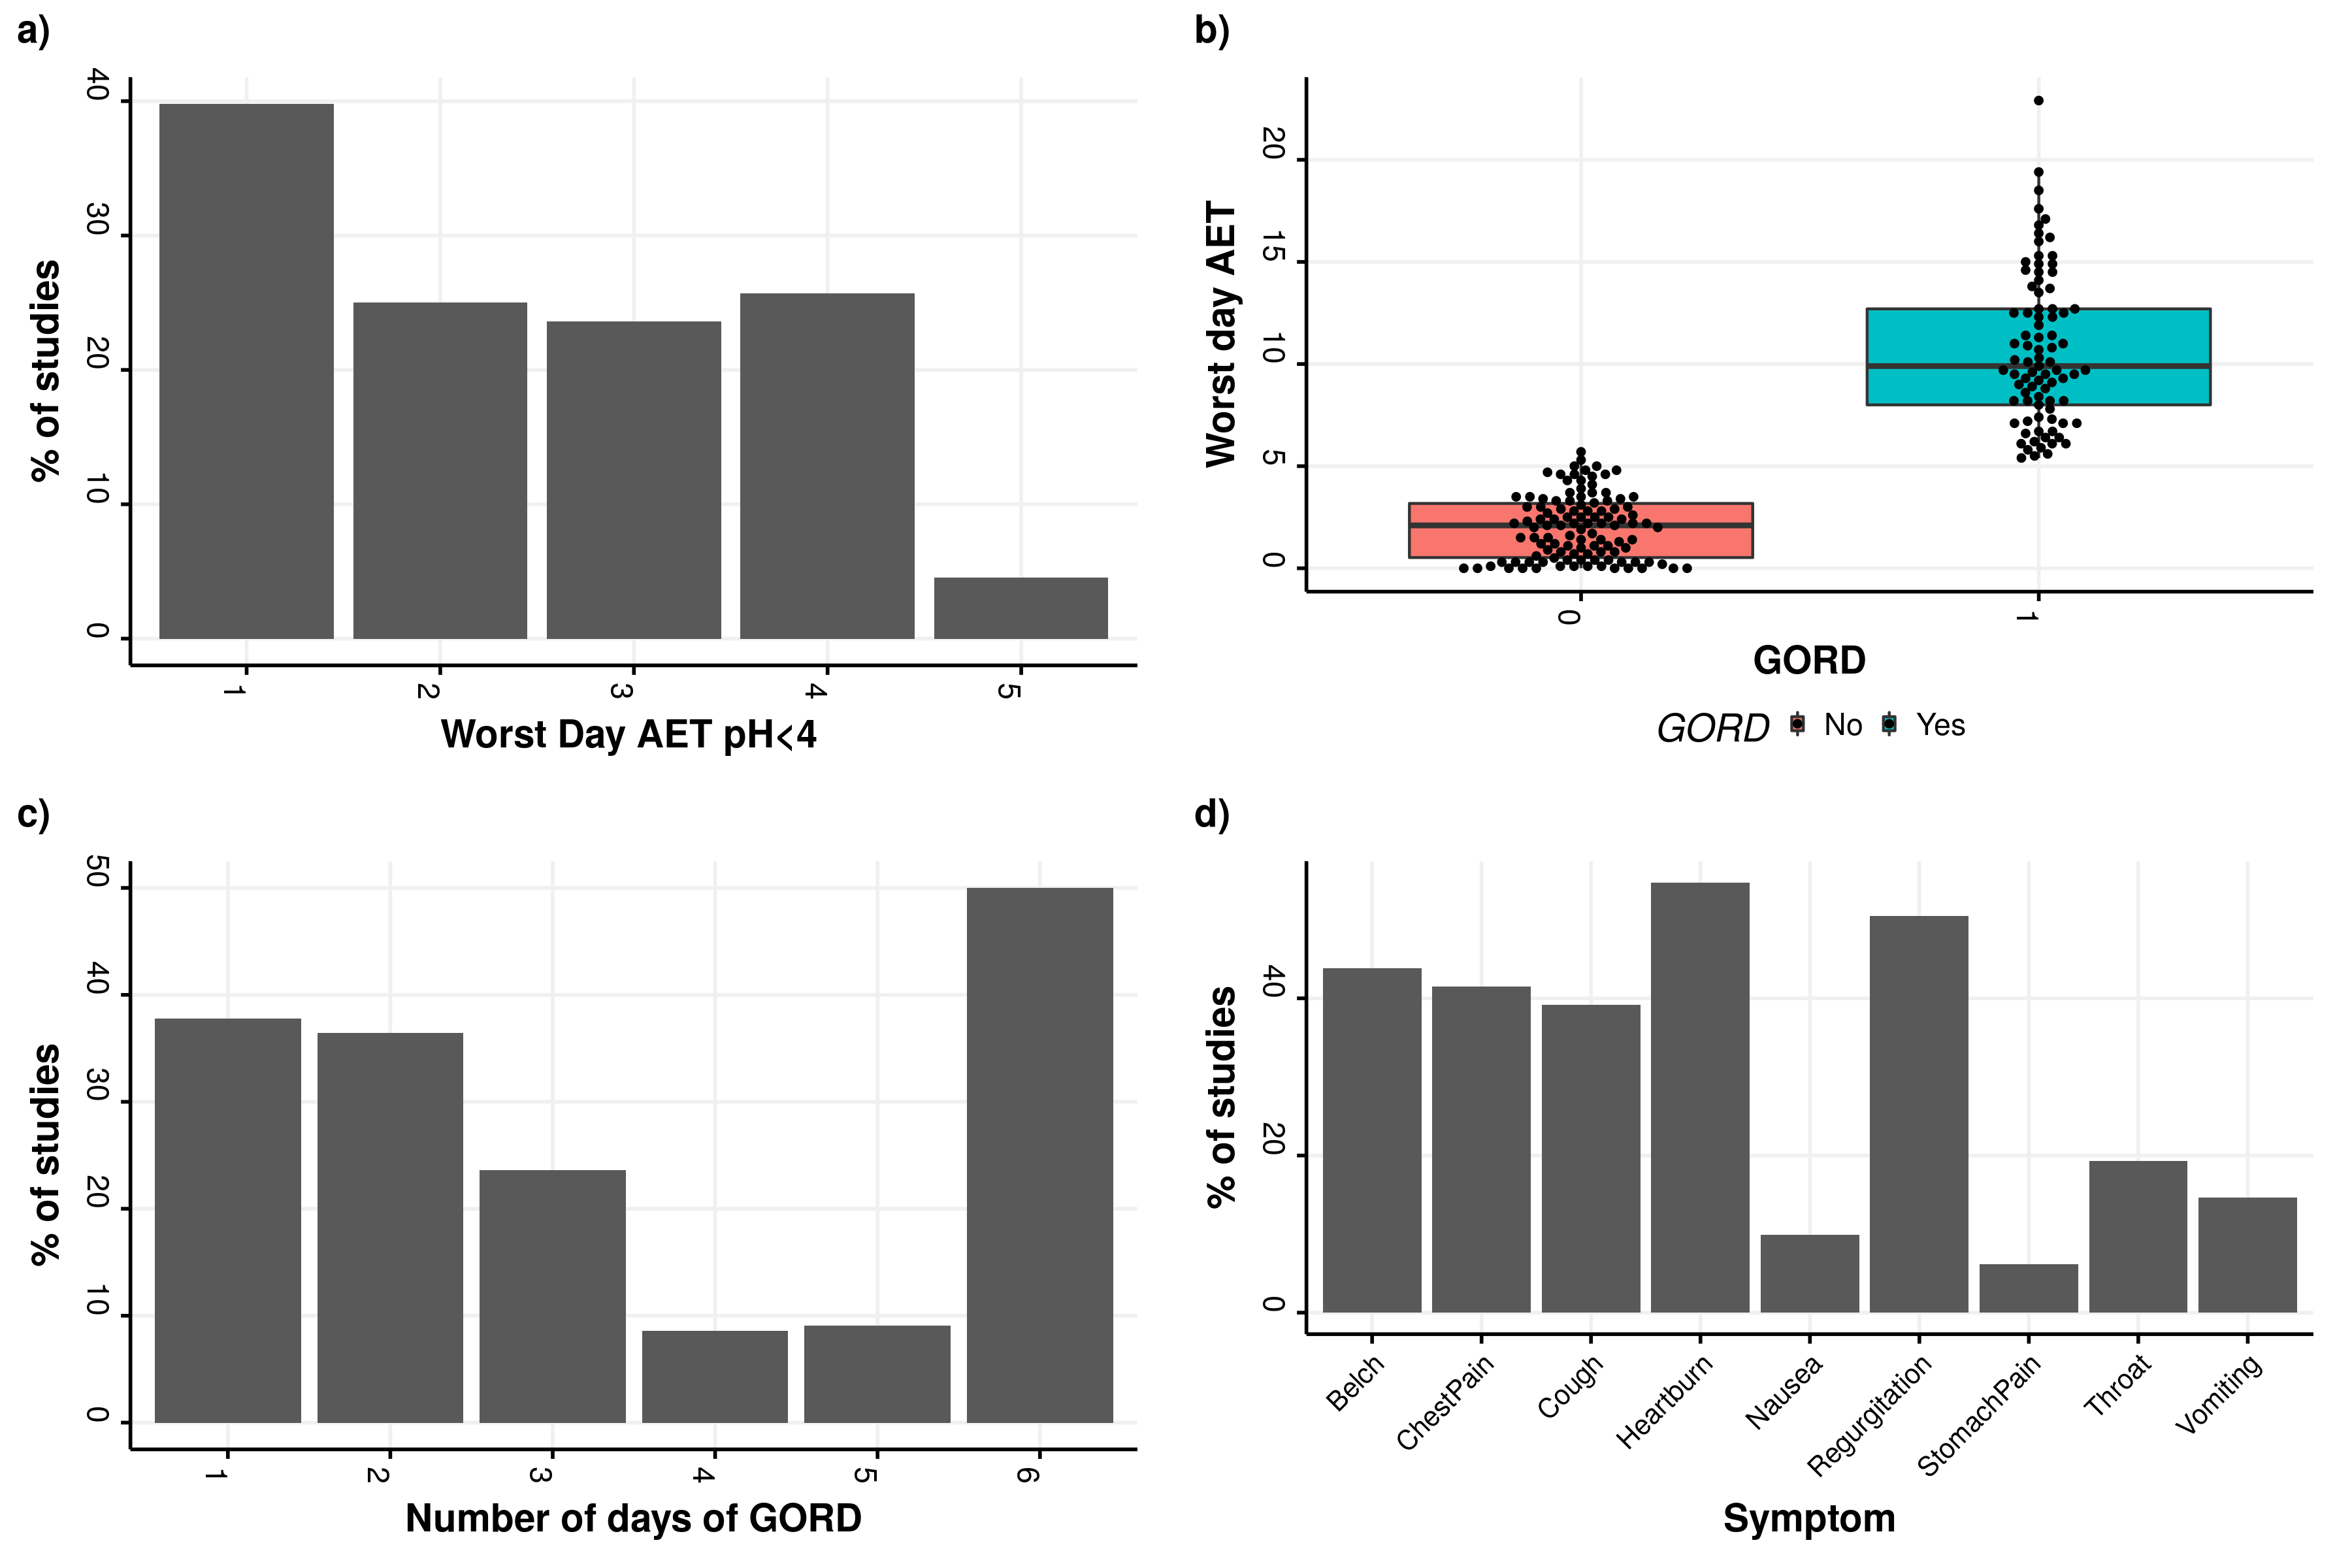
\includegraphics{TemplateReport_files/figure-latex/BRAVOdescription-1} \hfill{}

\caption{The characteristics of GORD positive WPM recordings for patients with negative impedance studies. a) Histogram of the worst day for WPM-GORD positive patients presented as a proportion of patients who completed a study in that day b) The percentage acid exposure time for WPM-GORD positive and WPM-GORD negative studies c) The number of days with GORD for GORD positive WPM studies expressed as a proportion of patients who completed the study for at least those number of days. d) The symptoms registered by patients as a percentage of all BRAVO epsisodes}\label{fig:BRAVOdescription}
\end{figure}

\begin{verbatim}
FALSE [1] "Error in binom.test(nn[i, j], n.ij, conf.level = conf.level) : \n  'n' must be a positive integer >= 'x'\n"
FALSE attr(,"class")
FALSE [1] "try-error"
FALSE attr(,"condition")
FALSE <simpleError in binom.test(nn[i, j], n.ij, conf.level = conf.level): 'n' must be a positive integer >= 'x'>
FALSE [1] "Error in binom.test(nn[i, j], n.ij, conf.level = conf.level) : \n  'n' must be a positive integer >= 'x'\n"
FALSE attr(,"class")
FALSE [1] "try-error"
FALSE attr(,"condition")
FALSE <simpleError in binom.test(nn[i, j], n.ij, conf.level = conf.level): 'n' must be a positive integer >= 'x'>
FALSE [1] "Error in binom.test(nn[i, j], n.ij, conf.level = conf.level) : \n  'n' must be a positive integer >= 'x'\n"
FALSE attr(,"class")
FALSE [1] "try-error"
FALSE attr(,"condition")
FALSE <simpleError in binom.test(nn[i, j], n.ij, conf.level = conf.level): 'n' must be a positive integer >= 'x'>
FALSE [1] "Error in binom.test(nn[i, j], n.ij, conf.level = conf.level) : \n  'n' must be a positive integer >= 'x'\n"
FALSE attr(,"class")
FALSE [1] "try-error"
FALSE attr(,"condition")
FALSE <simpleError in binom.test(nn[i, j], n.ij, conf.level = conf.level): 'n' must be a positive integer >= 'x'>
\end{verbatim}

\captionsetup[table]{labelformat=empty,skip=1pt}
\begin{longtable}{lccc}
\toprule
\textbf{Characteristic}\textsuperscript{1} & \textbf{Negative}, N = 113 (53\%) & \textbf{Positive}, N = 99 (47\%) & \textbf{p-value}\textsuperscript{2} \\ 
\midrule
Gender &  &  & 0.50 \\ 
Female & 69 / 113 (61\%) & 55 / 99 (56\%) &  \\ 
Male & 44 / 113 (39\%) & 44 / 99 (44\%) &  \\ 
LES midpoint from nares (cm) & 43.8 (3.4) & 43.5 (3.4) & 0.31 \\ 
Basal resp. min. (mmHg) & 11 (8) & 9 (10) & 0.004 \\ 
Residual mean (mmHg) & 6.0 (5.0) & 5.7 (6.1) & 0.28 \\ 
DCI (mean mmHg/cm/s) & 890 (783) & 741 (860) & 0.059 \\ 
Contractile front velocity (m/s) & 4.21 (5.77) & 4.04 (4.04) & 0.74 \\ 
Distal latency (s) & 7.14 (1.88) & 6.93 (1.26) & 0.89 \\ 
\% Failed peristalsis & 33 (33) & 36 (34) & 0.65 \\ 
\% Panoesophageal pressurization & 1.8 (5.9) & 2.2 (9.6) & 0.83 \\ 
\% Large Breaks & 7 (15) & 6 (12) & 0.88 \\ 
\% Small breaks & 14 (18) & 15 (17) & >0.99 \\ 
Number of Non acid episodes & 18 (18) & 21 (17) & 0.10 \\ 
Number of Acid Episodes & 13 (17) & 18 (16) & 0.036 \\ 
AET & 0.96 (0.99) & 1.54 (1.17) & <0.001 \\ 
Longest acid episode & 8 (11) & 8 (11) & 0.20 \\ 
Age (years) & 49 (14) & 47 (16) & 0.27 \\ 
Oesophagitis &  &  & 0.003 \\ 
N & 111 / 113 (98\%) & 86 / 99 (87\%) &  \\ 
Y & 2 / 113 (1.8\%) & 13 / 99 (13\%) &  \\ 
NA. &  &  & 0.83 \\ 
A & 1 / 2 (50\%) & 5 / 13 (38\%) &  \\ 
B & 1 / 2 (50\%) & 4 / 13 (31\%) &  \\ 
C & 0 / 2 (0\%) & 3 / 13 (23\%) &  \\ 
D & 0 / 2 (0\%) & 1 / 13 (7.7\%) &  \\ 
NA..1 &  &  &  \\ 
Unknown & 113 & 99 &  \\ 
NA..2 &  &  &  \\ 
2.8301886792452833 &  & 1 / 2 (50\%) &  \\ 
6 &  & 1 / 2 (50\%) &  \\ 
NA..3 &  &  &  \\ 
3.3018867924528301 &  & 1 / 2 (50\%) &  \\ 
7 &  & 1 / 2 (50\%) &  \\ 
NA..4 &  &  &  \\ 
1.4150943396226416 &  & 1 / 2 (50\%) &  \\ 
3 &  & 1 / 2 (50\%) &  \\ 
NA..5 &  &  &  \\ 
0.47169811320754718 &  & 1 / 2 (50\%) &  \\ 
1 &  & 1 / 2 (50\%) &  \\ 
SAP Heartburn &  &  & 0.71 \\ 
N & 53 / 113 (47\%) & 43 / 99 (43\%) &  \\ 
Y & 60 / 113 (53\%) & 56 / 99 (57\%) &  \\ 
SAP Chest Pain &  &  & 0.87 \\ 
N & 65 / 113 (58\%) & 59 / 99 (60\%) &  \\ 
Y & 48 / 113 (42\%) & 40 / 99 (40\%) &  \\ 
SAP Regurgitation &  &  & 0.69 \\ 
N & 54 / 113 (48\%) & 51 / 99 (52\%) &  \\ 
Y & 59 / 113 (52\%) & 48 / 99 (48\%) &  \\ 
SAP Belching &  &  & 0.77 \\ 
N & 65 / 113 (58\%) & 54 / 99 (55\%) &  \\ 
Y & 48 / 113 (42\%) & 45 / 99 (45\%) &  \\ 
SAP Cough &  &  & 0.36 \\ 
N & 65 / 113 (58\%) & 64 / 99 (65\%) &  \\ 
Y & 48 / 113 (42\%) & 35 / 99 (35\%) &  \\ 
SAP Throat Symptoms &  &  & 0.82 \\ 
N & 90 / 113 (80\%) & 81 / 99 (82\%) &  \\ 
Y & 23 / 113 (20\%) & 18 / 99 (18\%) &  \\ 
SAP Stomach pain &  &  & 0.22 \\ 
N & 113 / 113 (100\%) & 97 / 99 (98\%) &  \\ 
Y & 0 / 113 (0\%) & 2 / 99 (2.0\%) &  \\ 
SAP Vomiting &  &  & >0.99 \\ 
N & 98 / 113 (87\%) & 86 / 99 (87\%) &  \\ 
Y & 15 / 113 (13\%) & 13 / 99 (13\%) &  \\ 
SAPTotalNausea & 57 (47) & 58 (48) & 0.53 \\ 
\bottomrule
\end{longtable}
\vspace{-5mm}
\begin{minipage}{\linewidth}
\textsuperscript{1}Statistics presented: n / N (\%); mean (SD) \\ 
\textsuperscript{2}Statistical tests performed: chi-square test of independence; Wilcoxon rank-sum test; Fisher\textquotesingle{}s exact test \\ 
\end{minipage}

\hypertarget{baseline-demographic-data}{%
\subsubsection{Baseline demographic data}\label{baseline-demographic-data}}

Of the 212 included, 99 studies were positive for GORD (Male:Female 44: 55, average age of 47 (16) years and
113 negative for GORD (Male:Female 44: 69 average age of 49 (14) years).

The fraction of time with pH\textless{}4 (acid exposure time, AET), measured at WPM, is shown in Figure 1. Worst day analysis demonstrated a positive skew towards a GORD diagnosis on the first day. 37 (37.76)\% of patients classified as WPM-GORD-positive were positive for only 1 day. Of those diagnoses, 13 patients were positive on the first day. For patients who only had one day of GORD, the extra number of GORD diagnoses on day 2, 3 and 4 of WPM was 10,9 and 5 patients respectively. The number of studies that were negative for GORD in the first 24 hours and 48 hours of the WPM study was 22 (22.22 \% and 19 (19.19\%) respectively. The worst day symptom association probability (SAP) was positive in 63.68\%. The majority of the worst SAP days occurred in the first 24 hours for both positive and negative WPM studies.

\textbf{Table 1:} Table of demographics for GORD-positive (\enquote{Positive}) WPM and GORD-negative (\enquote{Negative}) WPM studies

\hypertarget{measures-of-contractile-vigour}{%
\subsubsection{Measures of contractile vigour}\label{measures-of-contractile-vigour}}

WPM-GORD-positive patients had no significant difference in DCI when compared with WPM-GORD-negative patients (WPM-GORD-positive patients (mmHg): 741 (860) vs.~WPM-GORD-negative patients (mmHg): 890 (783) p=0.059). There was no significant difference in the distal latency between the two groups (WPM-GORD-positive patients (s): 6.93 (1.26) vs.~WPM-GORD-negative patients (s): 7.14 (1.88) p=0.9.

No significant difference was observed between the two groups for large breaks (WPM-GORD-positive (\%): 6 (12) WPM-GORD-negative (\%): 7 (15), p=0.9) or for small breaks (WPM-GORD-positive (\%): 15 (17) WPM-GORD-negative (\%): 14 (18), p\textgreater{}0.9). Similarly there was no difference between the two groups in measurements of Contractile front velocity (WPM-GORD-positive (cm/s): 4.04 (4.04) WPM-GORD-negative (cm/s): 4.21 (5.77), p=0.7) or panoesophageal pressurization: (WPM-GORD-positive (\%): 2.2 (9.6) WPM-GORD-negative (\%): 1.8 (5.9), p=0.8)

\hypertarget{measures-of-lower-oesophageal-sphincter}{%
\subsubsection{Measures of lower oesophageal sphincter}\label{measures-of-lower-oesophageal-sphincter}}

There was a significant difference in the basal respiratory minimum (mmHg) between the two groups (WPM-GORD-positive (mmHg): 9 (10) vs WPM-GORD-negative (mmHg): 11 (8) p=0.004 ). A lack of significant difference was noted for the residual mean (mmHg) between the two groups (WPM-GORD-positive (mmHg): 5.7 (6.1) vs WPM-GORD-negative (mmHg): 6.0 (5.0) p=0.3 )

\hypertarget{ph-impedance-measurements}{%
\subsubsection{pH Impedance measurements}\label{ph-impedance-measurements}}

WPM-GORD-positive patients had a longer AET at pH impedance when compared with WPM-GORD-negative patients (WPM-GORD-positive patients (\%): 1.54 (1.17) vs.~WPM-GORD-negative patients (\%): 0.96 (0.99) p\textless{}0.001).

The AET when measured in an upright position was significantly increased in WPM-GORD-positive patients when compared with the WPM-GORD-negative group (p=0.001). There was no difference in supine reflux (data not shown). The longest time spent in reflux did not show any significant difference although the number of refluxes was significantly increased in the WPM-GORD-positive group 18 (16) vs.~13 (17) p=0.036.

\hypertarget{symptoms-and-endoscopic-findings}{%
\subsubsection{Symptoms and endoscopic findings}\label{symptoms-and-endoscopic-findings}}

The SAP did not differ for any of the individual symptoms (heartburn, chest pain, regurgitation, belching, cough, throat symptoms, abdominal pain, vomiting, nausea) between the two groups. Oesophagitis was more common in the WPM-GORD-Positive group 13.10\% vs.~1.80\%. Of these patients, the patients were graded as Los Angeles grade A,B,C or D in 2.8\%, 3.3\%, 1.4\% and 0.5\% respectively.
Univariate analysis highlighted Basal resp. min. (mmHg), Number of Acid Episodes,AET and Oesophagitis for further investigation with a multivariate analysis

\pagebreak

\pagebreak

\begin{figure}

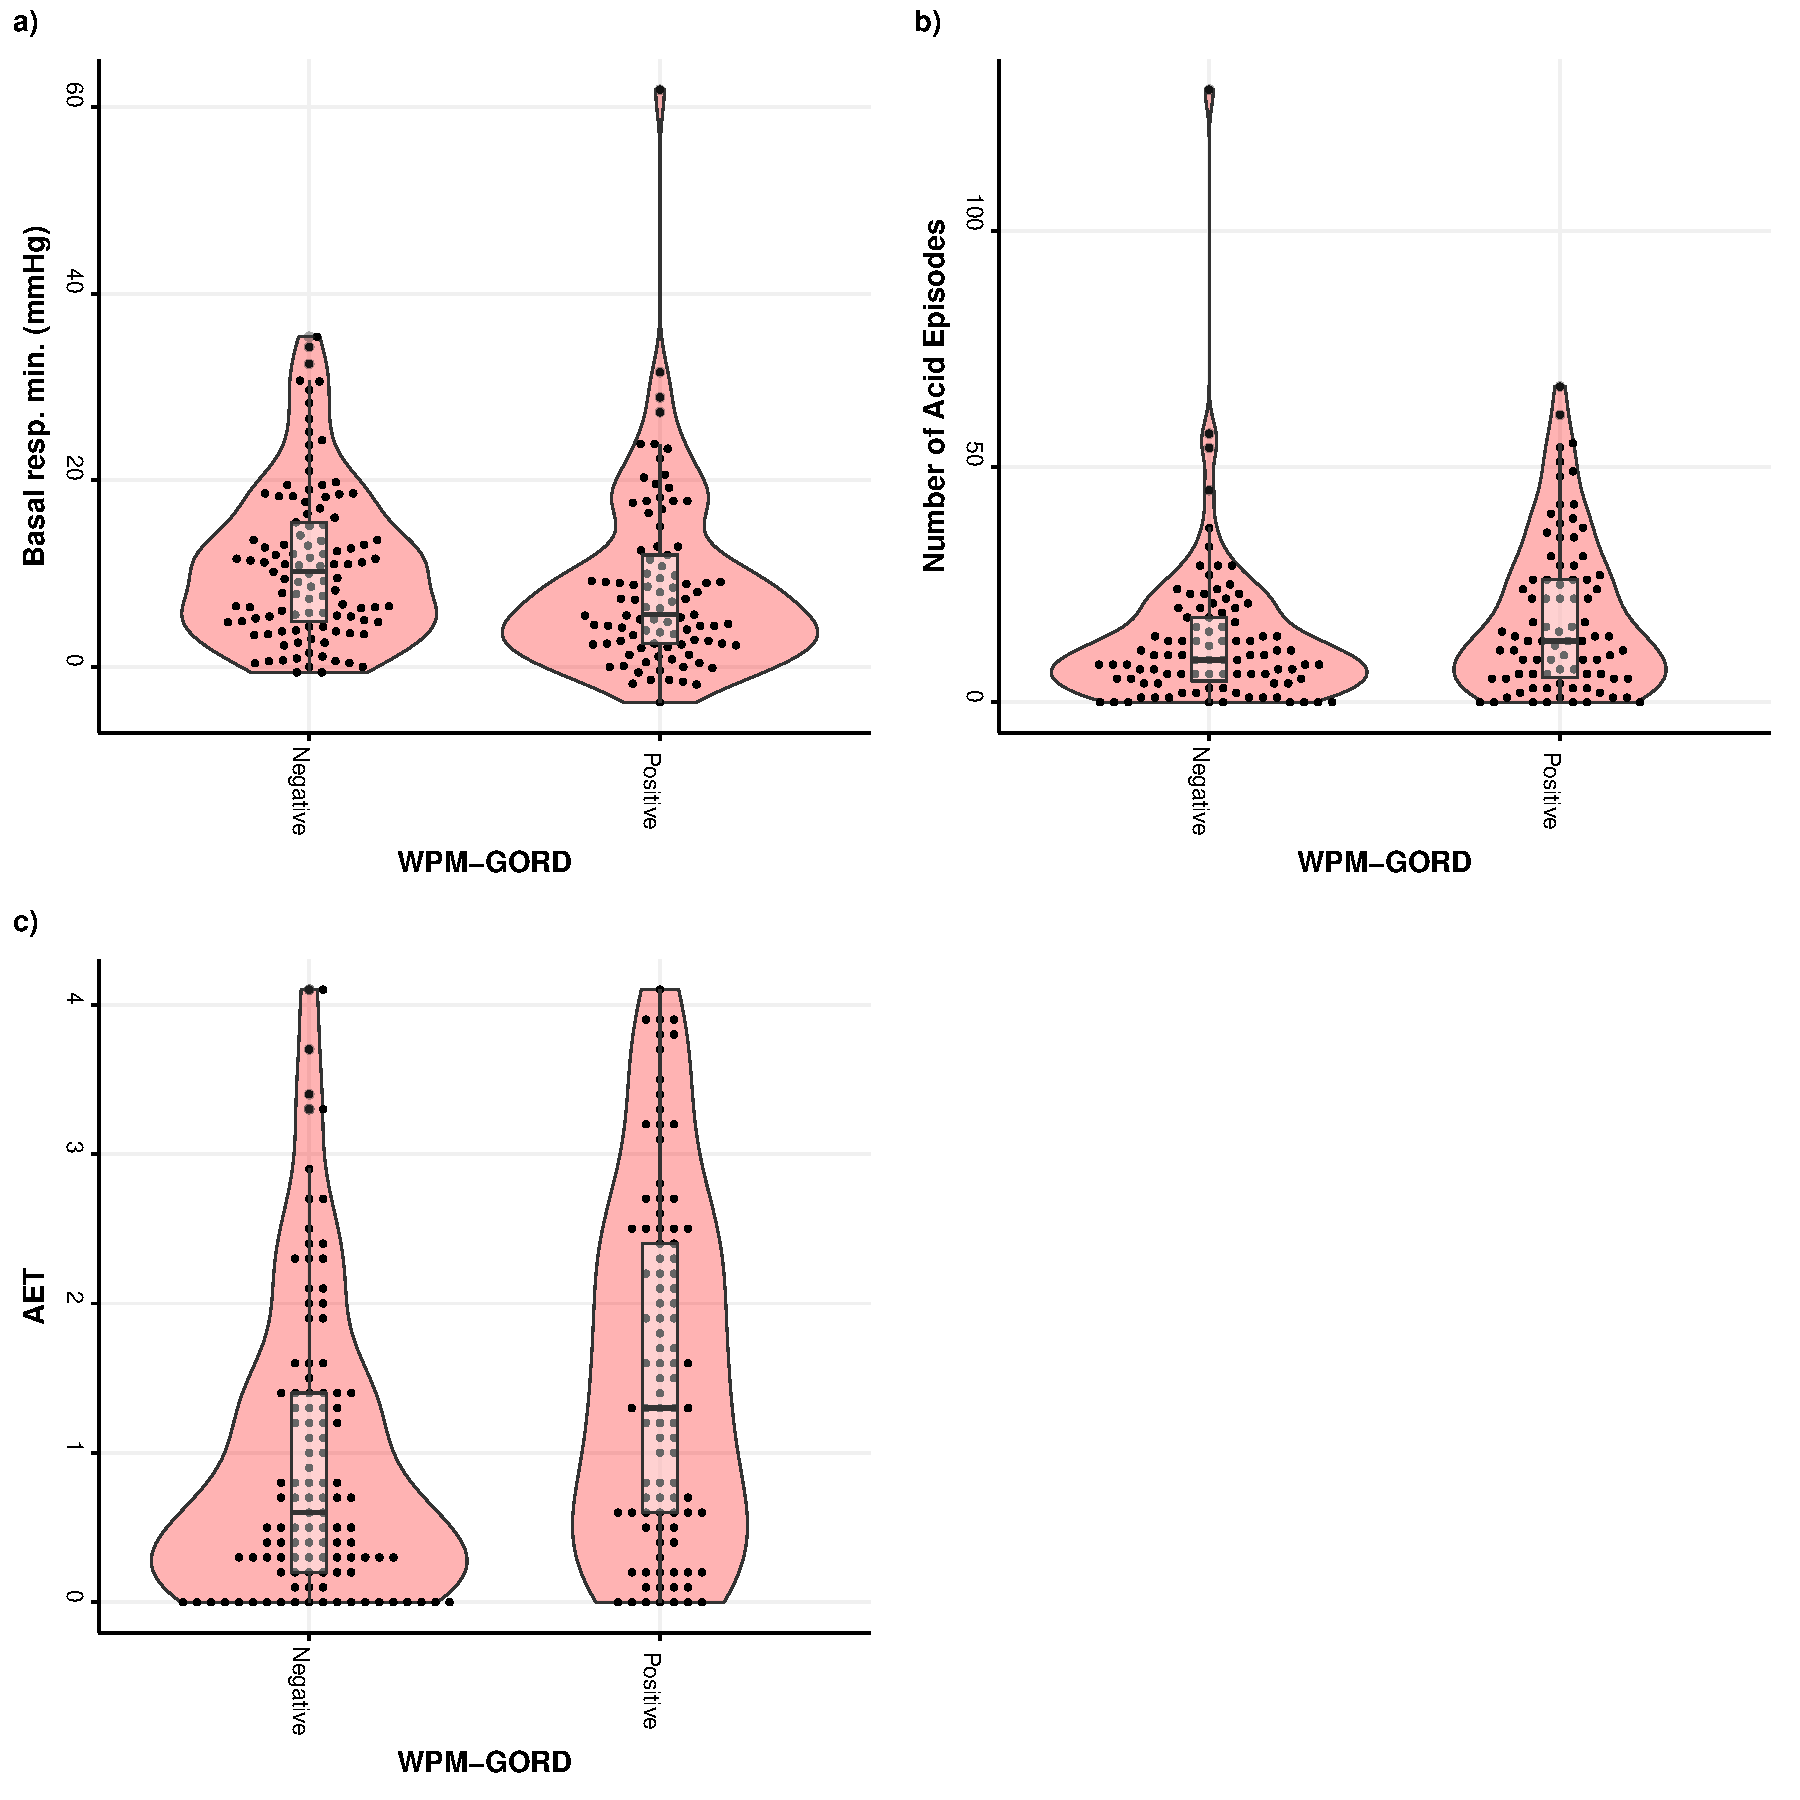
\includegraphics{TemplateReport_files/figure-latex/UnivariatePredictorsGraph-1} \hfill{}

\caption{pH impedance characteristics for predictors of a positive wireless capsule study for pH impedance negative studies. a) Basal respiratory minimum (mmHg)  b) Number of acid episodes c) Percentage time pH <4}\label{fig:UnivariatePredictorsGraph}
\end{figure}

\pagebreak

\hypertarget{multivariate-analysis}{%
\subsection{Multivariate analysis:}\label{multivariate-analysis}}

\textbf{Table 2:} Table of multivariate analysis to assess pH impedance and manometry variables from the univariate analysis.

\captionsetup[table]{labelformat=empty,skip=1pt}
\begin{longtable}{lccc}
\toprule
\textbf{Characteristic} & \textbf{OR}\textsuperscript{1} & \textbf{95\% CI}\textsuperscript{1} & \textbf{p-value} \\ 
\midrule
Basal resp. min. (mmHg) & 0.98 & 0.95, 1.02 & 0.4 \\ 
Number of Acid Episodes & 0.99 & 0.96, 1.02 & 0.6 \\ 
AET & 1.66 & 1.10, 2.56 & 0.018 \\ 
Oesophagitis & 5.01 & 1.21, 34.1 & 0.047 \\ 
\bottomrule
\end{longtable}
\vspace{-5mm}
\begin{minipage}{\linewidth}
\textsuperscript{1}OR = Odds Ratio, CI = Confidence Interval \\ 
\end{minipage}

A stepwise multiple logistic regression analysis was performed where the independent variables were those being analysed and the dependent variable was the presence of pathological acid reflux on a WPM study (\textbf{Table 2}). Variables chosen were those found to be significantly different in the univariate analysis. The AET at pH impedance was found to be a significant predictor of a positive WPM study: OR:1.66 (1.10-2.56, p=0.018). Oesophagitis at the point of BRAVO insertion was also a significant predictor of GORD on mutivariate analysis OR: 5.01 (1.21-34.09, p=0.047)

\newpage

\begin{figure}
\centering
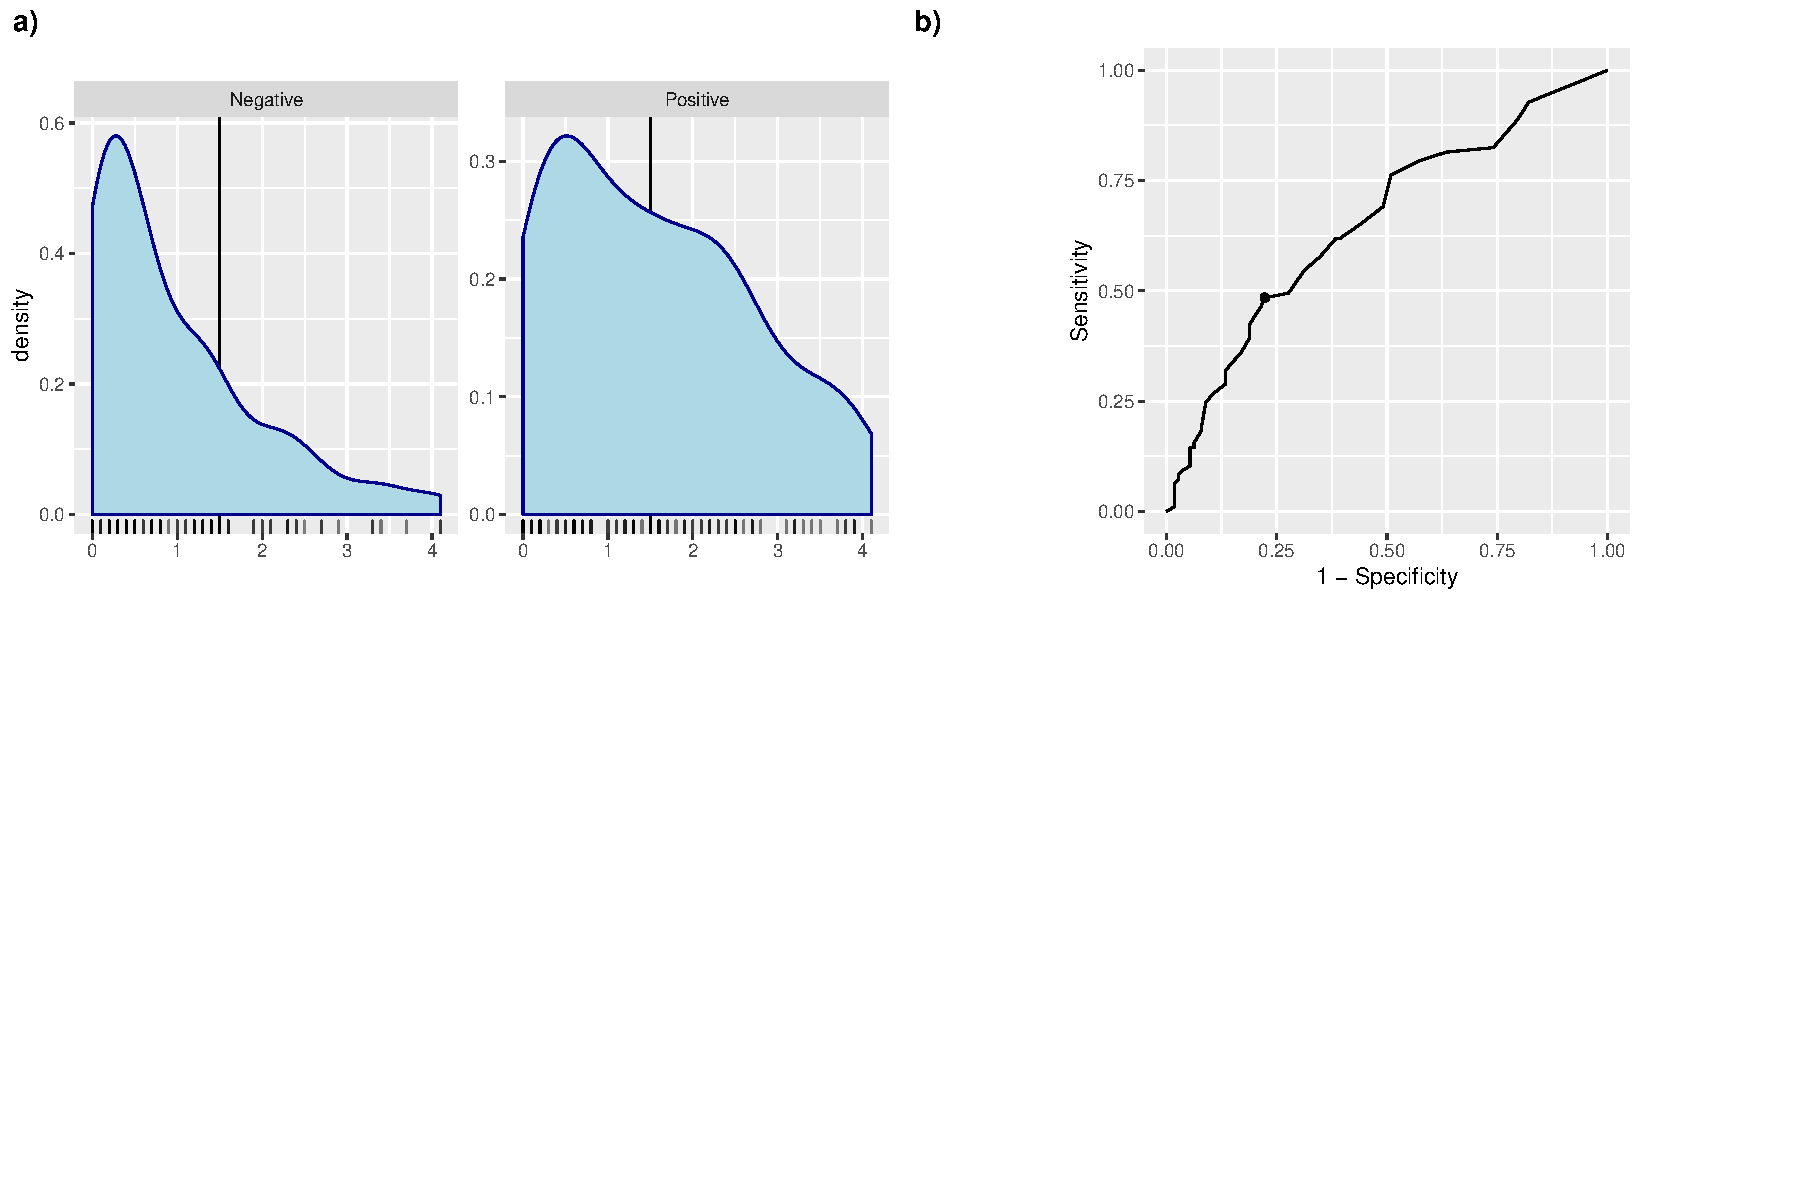
\includegraphics{TemplateReport_files/figure-latex/CutPointForAcid-1.pdf}
\caption{\label{fig:CutPointForAcid}Optimal cutpoint with distribution by class and associated ROC curve analysis a) Denisity plot showing the ability to discriminate positive and negative tests given the calculated cutpoint for Acid Exposure time (\%) b) ROC curve for the Acid exposure time (\%)}
\end{figure}

Given that AET can predict a positive WPM, Youden's cutpoint estimation determined that an AET of 1.50 gave a sensitivity of 48.45 \% and a specificity of 77.68 \% for the prediction of a positive subsequent WPM study. A ROC curve analysis demonstrated an area under the curve of 0.65, (sensitivity: 0.48\%,specificity:0.78,accuracy:0.64 (Figure 3).

\hypertarget{discussion}{%
\section{Discussion}\label{discussion}}

The current study represents the largest cohort of pH impedance GORD-negative patients who subsequently underwent WPM testing at the clinician's discretion. This cohort is unique in that the experience of increased positive diagnosis yield made with wireless pH studies is replicated for the first time with pH impedance as opposed to standard pH studies. It is notable that the WPM studies have shown a distribution of positivity similar to previous studies: the diagnosis of GORD is most often made on the basis of one day of positivity and of those patients who are positive for GORD, the worst day analysis is predominantly on the first day. (Sweis et al., 2011). Furthermore a significant number of WPM studies were positive after a negative impedance study. This has been noted on previous studies (Sweis et al., 2011) and may be related to the extended monitoring time (J. Pandolfino, 2003).

The increased yield of wireless pH as compared with standard pH studies has been demonstrated previously (Scarpulla et al., 2007). The reasons for the increased yield may be multifactorial including increased patient tolerability (Wong et al., 2005) and better detection of intermittent reflux episodes. In this current study, of the patients who turn out to be GORD positive, the number of patients who were GORD negative in the first 24 hours was 22.22\%. A further 19.19\% were still negative after 48 hours indicating that even a 48 hour pH study may be insufficient. The number of patients who were GORD positive on only one day also argues for monitoring for longer than 24 hours as it suggests that a significant number of GORD positive patients in this cohort may have intermittent symptoms.

The fact that there is an increased yield with prolonged monitoring is important for two reasons. Firstly, it highlights the possibility that a pH impedance study may be a false negative which increases the chance that a clinician may refer on for a prolonged WPM study subsequently. Secondly, pH impedance is time consuming when compared to BRAVO analysis and standard pH analysis; the analysis of much of the two latter studies can be automated in a way that is not possible with pH impedance. Given the increased patient comfort and tolerability associated with WPM studies (Wong et al., 2005), automation of the much of the analysis, the ability to perform an endoscopic examination during capsule placement and the increased positive diagnosis yield, there may be a strong case for further clinical studies assessing the use of WPM as a first line investigation instead of standard 24 hour pH or 24 hour pH impedance monitoring.

The fact that most motility variables were not associated with WPM GORD-positivity is in keeping with the established literature that there is no specific pattern at HRM that predicts the presence of GORD. There are findings however that are more likely in GORD. Distal contractile integral (DCI), a measure of contractile vigour, has been shown to be lower in GORD patients (Hoeij, Smout, \& Bredenoord, 2015) although in mild ineffective oesophageal motility the relationship to GORD is less well proven ((Fornari et al., 2007)) Univariate analysis has only shown a tendency towards significance for the DCI between the two groups although multivariate analysis did not demonstrate this to be a significant discriminator. A reduced basal respiratory minimum pressure is also known to be associated with increasing severity of GORD ((Savarino et al., 2011)) as has been found in this study. Again this was not found to be an important factor on the multivariate analysis. The fact that this is the case for both DCI and the basal respiratory minimum may be related to the study population. 37\% of patients positive for GORD by WPM were only positive on one day indicating the intermittent nature of reflux in a proportion of this cohort. Furthermore most of the patients did not have erosive oesophagitis. The DCI is well documented to be more severely affected in patients with oesophagitis and motility disorders are more commonly seen as patients progress from non-erosive reflux disease to increasing severity of GORD to Barrett's oesophagus (Savarino et al., 2011). The study population therefore represents a GORD population less likely to have motility dysfunction. That the presence of oesophagitis is a predictor of a positive WPM is not surprising. Arguably, the presence of oesophagitis at endoscopy should preclude the need for further pH testing (although in this study the oesophagitis was diagnosed at the point of WPM insertion) so that this should not be used as a predictor of a subsequent WPM study.

The significant difference in the acid exposure time at pH impedance, between those who have GORD at WPM and those who do not is interesting. Some false negative pH studies may be related to patients altering their behaviour because of the presence of a nasal catheter (Fass et al., 1999) therefore reducing the AET into the normal range. It is also possible that the cohort in this study represent more borderline GORD diagnoses making the ability to use predictors more difficult. This significant difference does not translate in to a value with sufficient accuracy to allow physicians to determine who should go on to have a WPM study. Furthermore, no other measurement taken at impedance, including parameters of non-acid reflux, are relevant albeit in this selected group.

The decision to submit a patient to a WPM study following a negative pH impedance study may be more likely in those who have typical and convincing symptoms. Typical GORD symptoms such as regurgitation and heartburn are well documented to be better predictors of oesophagitis than atypical symptoms (\textbf{\url{https://doi.org/10.1016/j.gtc.2013.11.002}}). It is therefore a surprise that symptoms do not predict the presence of GORD. This may be because the symptom was user-defined as it was recorded by the patient. Patient-defined features do not always correlate well with questionnaire defined symptoms.

The study is limited insofar as it is retrospective and the selection criteria for those who were selected for WPM were at the physician's discretion. Also, as noted above, patient defined symptoms may be difficult to interpret. However the patient cohort does represent a real-world selection at a high throughput centre.

In conclusion this study demonstrates that there is a significant increase in positive GORD diagnosis yield in patients with a negative pH impedance in a cohort selected on clinical suspicion for further testing. It is difficult to determine which patients may benefit from prolonged oesophageal pH monitoring in the context of a negative 24 hour pH impedance test. There is no single factor that reliably distinguishes those who will and will not have GORD on WPM with sufficient sensitivity and specificity. The presence of oesophagitis at endoscopy should indicate that a further period of monitoring is not necessary rather than act as an indicator for further testing. The combination of increased diagnostic yield and the inability to accurately predict who will have a positive extended WPM could strengthen the argument for a more formal assessment of WPM as the first line investigation in patients who require a positive diagnosis of GORD.

\hypertarget{data-analysis}{%
\subsection{Data analysis}\label{data-analysis}}

We used R {[}Version 3.6.0; @{]} and the R-packages \emph{EndoMineR} (Version 2.0.1.9000; Zeki, 2018a, 2018a), and \emph{PhysiMineR} (Version 0.0.0.9000; Zeki, 2018b, 2018b) for all our analyses.

\newpage

\hypertarget{author-contribution}{%
\section{Author contribution}\label{author-contribution}}

Sebastian Zeki,Jafar Jafari,Guiping Sui,Ismail Miah,Minerva daSilva,Anna Wolak: acquisition of data, Andrew Davies, Abrie Botha, Terry Wong, Jafar Jafari: data analysis and interpretation, Sebastian Zeki: statistical analysis, drafting of the manuscript; Jafar Jafari, Guiping Sui, Ismail Miah, Minerva daSilva, Anna Wolak, Jason Dunn, Andrew Davies, James Gossage, Abrie Botha, Terry Wong: critical revision of the manuscript for important intellectual content.

\hypertarget{references}{%
\section{References}\label{references}}

\begingroup
\setlength{\parindent}{-0.5in}
\setlength{\leftskip}{0.5in}

\hypertarget{refs}{}
\leavevmode\hypertarget{ref-Fass1999}{}%
Fass, R., Hell, R., Sampliner, R. E., Pulliam, G., Graver, E., Hartz, V., \ldots{} Jaffe, P. (1999). Effect of ambulatory 24-hour esophageal pH monitoring on reflux-provoking activities. \emph{Digestive Diseases and Sciences}, \emph{44}(11), 2263--2269. \url{https://doi.org/10.1023/a:1026608804938}

\leavevmode\hypertarget{ref-FORNARI2007}{}%
Fornari, F., Blondeau, K., Durand, L., Rey, E., Diaz-Rubio, M., De Meyer, A., \ldots{} Sifrim, D. (2007). Relevance of mild ineffective oesophageal motility (IOM) and potential pharmacological reversibility of severe IOM in patients with gastro-oesophageal reflux disease. \emph{Alimentary Pharmacology \& Therapeutics}, \emph{26}(10), 1345--1354. \url{https://doi.org/10.1111/j.1365-2036.2007.03525.x}

\leavevmode\hypertarget{ref-Gyawali2018}{}%
Gyawali, C. P., Kahrilas, P. J., Savarino, E., Zerbib, F., Mion, F., Smout, A. J. P. M., \ldots{} Roman, S. (2018). Modern diagnosis of GERD: the Lyon Consensus. \emph{Gut}, \emph{67}(7), 1351--1362. \url{https://doi.org/10.1136/gutjnl-2017-314722}

\leavevmode\hypertarget{ref-VanHoeij2015}{}%
Hoeij, F. B. van, Smout, A. J., \& Bredenoord, A. J. (2015). Predictive value of routine esophageal high-resolution manometry for gastro-esophageal reflux disease. \emph{Neurogastroenterology \& Motility}, \emph{27}(7), 963--970. \url{https://doi.org/10.1111/nmo.12570}

\leavevmode\hypertarget{ref-Kahrilas2015}{}%
Kahrilas, P. J., Bredenoord, A. J., Fox, M., Gyawali, C. P., Roman, S., Smout, A. J. P. M., \& Pandolfino, J. E. (2015). The Chicago Classification of esophageal motility disorders, v3.0. \emph{Neurogastroenterology \& Motility}, \emph{27}(2), 160--174. \url{https://doi.org/10.1111/nmo.12477}

\leavevmode\hypertarget{ref-Pandolfino2003a}{}%
Pandolfino, J. (2003). Ambulatory esophageal pH monitoring using a wireless system. \emph{The American Journal of Gastroenterology}, \emph{98}(4), 740--749. \url{https://doi.org/10.1016/S0002-9270(03)00062-5}

\leavevmode\hypertarget{ref-Pandolfino2003}{}%
Pandolfino, J. E., Richter, J. E., Ours, T., Guardino, J. M., Chapman, J., \& Kahrilas, P. J. (2003). Ambulatory esophageal pH monitoring using a wireless system. \emph{The American Journal of Gastroenterology}, \emph{98}(4), 740--749. \url{https://doi.org/10.1111/j.1572-0241.2003.07398.x}

\leavevmode\hypertarget{ref-Savarino2011}{}%
Savarino, E., Gemignani, L., Pohl, D., Zentilin, P., Dulbecco, P., Assandri, L., \ldots{} Savarino, V. (2011). Oesophageal motility and bolus transit abnormalities increase in parallel with the severity of gastro-oesophageal reflux disease. \emph{Alimentary Pharmacology \& Therapeutics}, \emph{34}(4), 476--486. \url{https://doi.org/10.1111/j.1365-2036.2011.04742.x}

\leavevmode\hypertarget{ref-Scarpulla2007a}{}%
Scarpulla, G., Camilleri, S., Galante, P., Manganaro, M., \& Fox, M. (2007). The Impact of Prolonged pH Measurements on the Diagnosis of Gastroesophageal Reflux Disease: 4-Day Wireless pH Studies. \emph{The American Journal of Gastroenterology}, \emph{102}(12), 2642--2647. \url{https://doi.org/10.1111/j.1572-0241.2007.01461.x}

\leavevmode\hypertarget{ref-Sweis2011}{}%
Sweis, R., Fox, M., Anggiansah, A., \& Wong, T. (2011). Prolonged, wireless pH-studies have a high diagnostic yield in patients with reflux symptoms and negative 24-h catheter-based pH-studies. \emph{Neurogastroenterology \& Motility}, \emph{23}(5), 419--426. \url{https://doi.org/10.1111/j.1365-2982.2010.01663.x}

\leavevmode\hypertarget{ref-Sweis2009}{}%
Sweis, R., Fox, M., Anggiansah, R., Anggiansah, A., Basavaraju, K., Canavan, R., \& Wong, T. (2009). Patient acceptance and clinical impact of Bravo monitoring in patients with previous failed catheter-based studies. \emph{Alimentary Pharmacology \& Therapeutics}, \emph{29}(6), 669--676. \url{https://doi.org/10.1111/j.1365-2036.2008.03923.x}

\leavevmode\hypertarget{ref-TSENG2005a}{}%
Tseng, D., A, R., Fennerty, M., Jobe, B., Diggs, B., Sheppard, B., \ldots{} Aye, R. (2005). Forty-Eight-Hour pH Monitoring Increases Sensitivity in Detecting Abnormal Esophageal Acid Exposure. \emph{Journal of Gastrointestinal Surgery}, \emph{9}(8), 1043--1052. \url{https://doi.org/10.1016/j.gassur.2005.07.011}

\leavevmode\hypertarget{ref-Wenner2005}{}%
Wenner, J., Johnsson, F., Johansson, J., \& Öberg, S. (2005). Wireless oesophageal pH monitoring: Feasibility, safety and normal values in healthy subjects. \emph{Scandinavian Journal of Gastroenterology}, \emph{40}(7), 768--774. \url{https://doi.org/10.1080/00365520510023602}

\leavevmode\hypertarget{ref-Wong2005a}{}%
Wong, W.-M., Bautista, J., Dekel, R., Malagon, I. B., Tuchinsky, I., Green, C., \ldots{} Fass, R. (2005). Feasibility and tolerability of transnasal/per-oral placement of the wireless pH capsule vs. traditional 24-h oesophageal pH monitoring - a randomized trial. \emph{Alimentary Pharmacology and Therapeutics}, \emph{21}(2), 155--163. \url{https://doi.org/10.1111/j.1365-2036.2005.02313.x}

\leavevmode\hypertarget{ref-R-EndoMineR}{}%
Zeki, S. (2018a). \emph{EndoMineR: Functions to mine endoscopic and associated pathology datasets}.

\leavevmode\hypertarget{ref-R-PhysiMineR}{}%
Zeki, S. (2018b). \emph{PhysiMineR: Functions to extract, clean, manipulate and analyse upper gastrointestinal physiological parameters}. Retrieved from \url{https://sebastiz.github.io/PhysiMineR/index.html}

\endgroup

\end{document}
